% --------------------------------------------------------------
% This is all preamble stuff that you don't have to worry about.
% Head down to where it says "Start here"
% --------------------------------------------------------------

\documentclass[12pt]{article}

\usepackage[margin=1in]{geometry}
\usepackage{amsmath,amsthm,amssymb}
\usepackage{graphicx} %This allows to include eps figures

% This is to include code
\usepackage{listings}
\usepackage{xcolor}
\definecolor{dkgreen}{rgb}{0,0.6,0}
\definecolor{gray}{rgb}{0.5,0.5,0.5}
\definecolor{mauve}{rgb}{0.58,0,0.82}
\lstdefinestyle{Python}{
    language        = Python,
    basicstyle      = \ttfamily,
    keywordstyle    = \color{blue},
    keywordstyle    = [2] \color{teal}, % just to check that it works
    stringstyle     = \color{green},
    commentstyle    = \color{red}\ttfamily
}

\newcommand{\N}{\mathbb{N}}
\newcommand{\Z}{\mathbb{Z}}

\newenvironment{theorem}[2][Theorem]{\begin{trivlist}
\item[\hskip \labelsep {\bfseries #1}\hskip \labelsep {\bfseries #2.}]}{\end{trivlist}}
\newenvironment{lemma}[2][Lemma]{\begin{trivlist}
\item[\hskip \labelsep {\bfseries #1}\hskip \labelsep {\bfseries #2.}]}{\end{trivlist}}
\newenvironment{exercise}[2][Exercise]{\begin{trivlist}
\item[\hskip \labelsep {\bfseries #1}\hskip \labelsep {\bfseries #2.}]}{\end{trivlist}}
\newenvironment{reflection}[2][Reflection]{\begin{trivlist}
\item[\hskip \labelsep {\bfseries #1}\hskip \labelsep {\bfseries #2.}]}{\end{trivlist}}
\newenvironment{proposition}[2][Proposition]{\begin{trivlist}
\item[\hskip \labelsep {\bfseries #1}\hskip \labelsep {\bfseries #2.}]}{\end{trivlist}}
\newenvironment{corollary}[2][Corollary]{\begin{trivlist}
\item[\hskip \labelsep {\bfseries #1}\hskip \labelsep {\bfseries #2.}]}{\end{trivlist}}

\begin{document}

% --------------------------------------------------------------
%                         Start here
% --------------------------------------------------------------

%\renewcommand{\qedsymbol}{\filledbox}

\title{Homework 2}%replace X with the appropriate number
\author{Thomas Buchegger\\ %replace with your name
Introduction to Signal and Image Processing}
\maketitle

\setcounter{tocdepth}3 % Set the depth of the table of contents to show sections and subsections only
\tableofcontents

\pagebreak
\section{Used Methods}
\subsection{Linear Filtering}
Linear filtering is used to modify a picture. This includes enhancing or removing features. Filtering is a so called neighbourhood operation, which means
that the value of a certain pixel is based on its neighbourhood pixels.
\newline
An example for a linear filter would be a box filter. It calculates the arithmetic means
based on its neighbourhood pixels for the new pixel. This leads to a blurring effect. 

\begin{figure}[!htb]
    \centering
    %omit extension of file. pdflatex will convert to pdf automatically.
    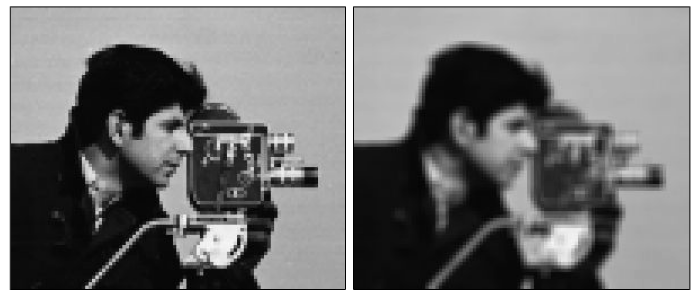
\includegraphics[width=0.8\textwidth]{pics/boxFilterExample}
    \caption{Filtering with a box-filter of size $3 \times 3$.}
    \label{fig:boxfilter}
    \end{figure}

\subsection{Finding edges}
As the name suggests, the goal is to detect edges in images.
One of the most popular edge detection algorithm is canny edge detection.
\newline
It consists of four steps:
\begin{enumerate}  
    \item Preprocessing with gauss for example
    \begin{figure}[!htb]
         \centering
         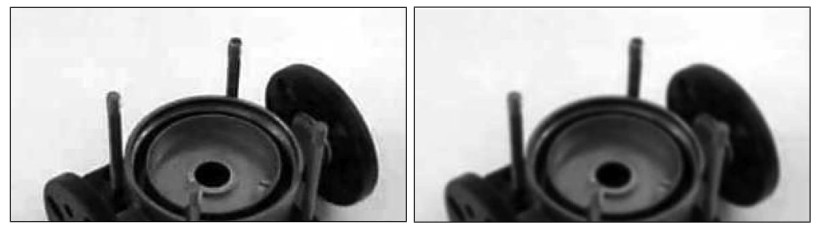
\includegraphics[width=0.8\textwidth]{pics/canny1}
         \caption{Before and after low pass filter}
         \label{fig:gaussfilter}
    \end{figure}

    \pagebreak
    \item Gradient calculation
    \begin{figure}[!htb]
        \centering
        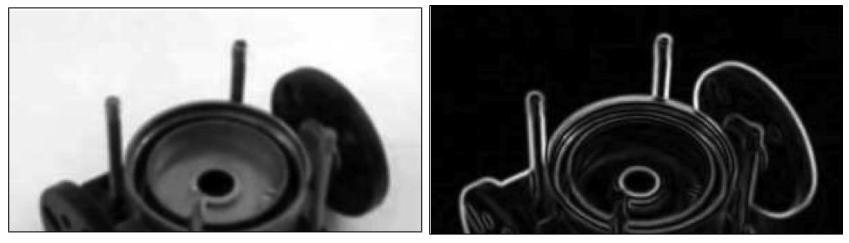
\includegraphics[width=0.8\textwidth]{pics/canny2}
        \caption{Before and after gradient calculation}
        \label{fig:gradients}
    \end{figure}

    \item Nonmax suppression
    \begin{figure}[!htb]
        \centering
        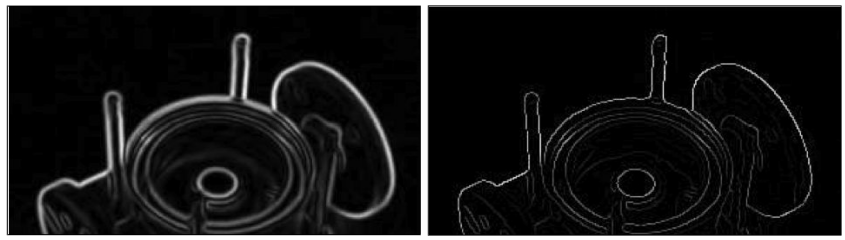
\includegraphics[width=0.8\textwidth]{pics/canny3}
        \caption{Before and after non max suppression} 
        \label{fig:nonmaxsuppression} 
    \end{figure}

    \item Hysteresis thresholding
    \begin{figure}[!htb]
        \centering
        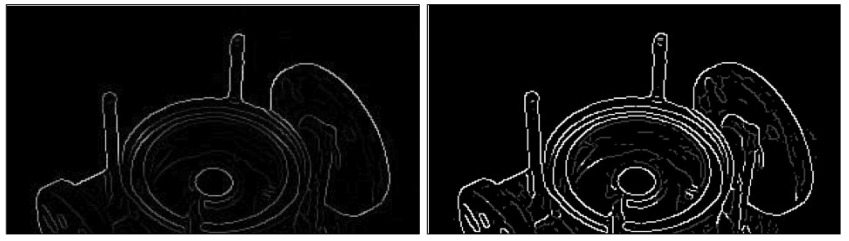
\includegraphics[width=0.8\textwidth]{pics/canny4}
        \caption{Before and after thresholding}
        \label{fig:thresholding}
    \end{figure}

    \end{enumerate}

\pagebreak
\subsection{Corner detection}
The goal is to detect corners in images. A corner is defined as an intersection
between two edges, as seen in figure 6.
    \begin{figure}[!htb]
        \centering
        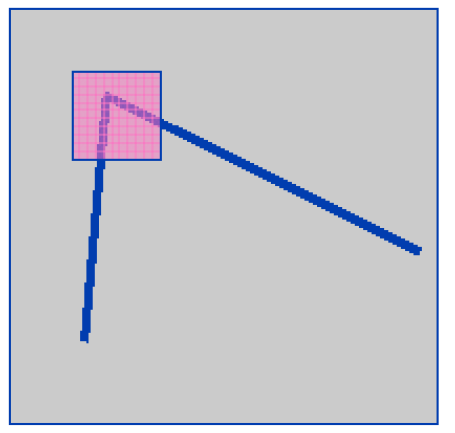
\includegraphics[width=0.5\textwidth]{pics/wellDefinedCorner}
        \caption{Corner as an intersection of two edges.}
        \label{fig:corners}
    \end{figure}

\section{Exercises}
\subsection{Linear Filtering}
\subsubsection{Boxfilter}
The function boxfilter(n) can be summarized as $np.ones((n, n)) / (n x n)$.

\subsubsection{myconv2}
The algorithm checks the dimensions first before proceeding and if nessecary, reshaping. After preparing the output,
a full convolution is made.

\pagebreak

\subsubsection{boxfilter with myconv2}
\begin{figure}[!htb]
    \centering
    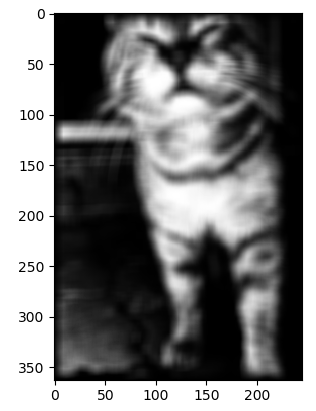
\includegraphics[width=0.5\textwidth]{pics/boxFilter10}
    \caption{Applied box filter size 10}
  \end{figure}

\subsubsection{gauss1d}
As described in the task, we using checks for making the filter odd. For performance reasons,
the numpy library with array multiplications and division is used.

\pagebreak
\subsubsection{gauss2d}
\begin{figure}[!htb]
    \centering
    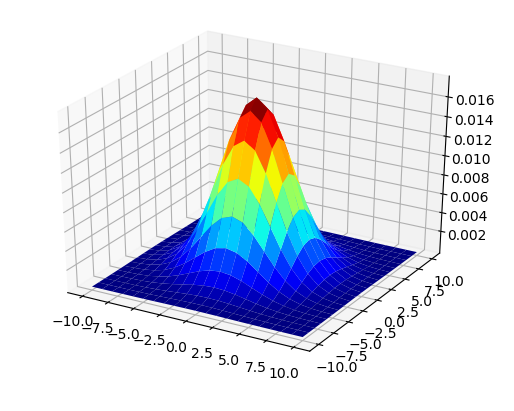
\includegraphics[width=0.5\textwidth]{pics/gaussPlot}
    \caption{Gaussian kernel in 3D space}
  \end{figure}
  Result of the Gaussian 1D and the $myconv$ function.

\subsubsection{gconv}
\begin{figure}[!htb]
  \centering
  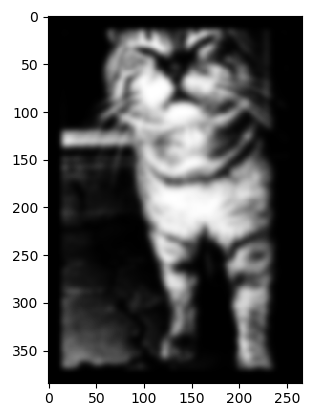
\includegraphics[width=0.4\textwidth]{pics/gaussFiltered}
  \caption{Result of the gaussian with sigma 3 on an image}
\end{figure}

\subsubsection{More efficient convolution}
The process of performing a convolution requires $K^2$ operations per pixel, where K is the size $(width == height == K)$ of the 
convolution kernel.In many cases, this operation can be speed up by first performing a 1D horizontal convolution followed by a 1D 
vertical convolution, requiring 2*K operations per pixel.If this is possible, then the convolution kernel is called separable!
Look at the singular value decomposition (SVD) of the kernel, and if only one singular value is non-zero, then it is separable.

\subsubsection{Computation time vs filter size experiment}
\begin{figure}[!htb]
    \centering
    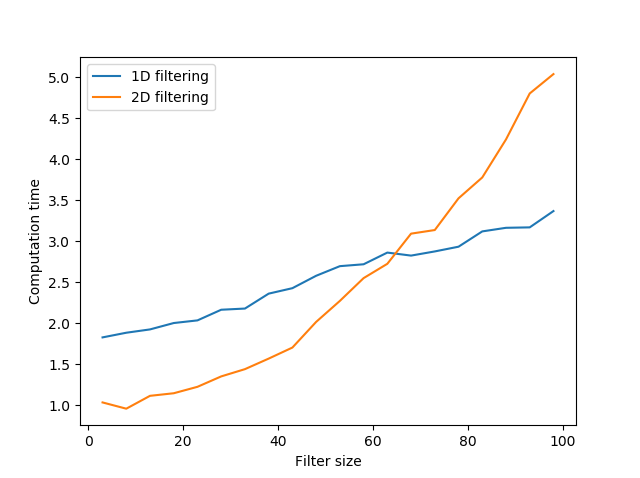
\includegraphics[width=0.8\textwidth]{pics/compTime}
    \caption{Compairson of 1D and 2D Gaus}
  \end{figure}
  The 2D filtering curve is much steeper, because of the factor 2 of
  the number of dimensions to be calculated.
  \newpage

\subsection{Finding edges}
\subsubsection{gradients}
Gradient detection is done with a high pass filter. In our excercise this is done with
once in x and once in y direction with the help of the $myconv2$ and $gauss1d$ functions.
The value for sigma is 1. 

\subsubsection{create edge magn image}
We only want the strongest edges in all directions, therefore we first define $direction_ranges$
in all eight directions. After that we iterate through the picture eight times - 
once in each direction. We then get the strongest and weakest gray value and
set only the strongest to 255, the rest to 0.

\begin{figure}[!htb]
    \centering
    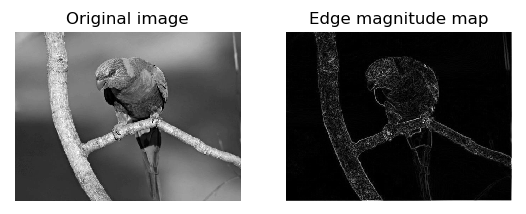
\includegraphics[width=0.8\textwidth]{pics/edgeMagnitudeMap}
    \caption{Original image and its magnitude map}
    \label{fig:magnitude}
\end{figure}

\subsubsection{make edge map}

\begin{figure}[!htb]
    \centering
    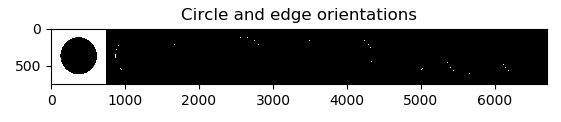
\includegraphics[width=0.8\textwidth]{pics/circleEdgeOrientation}
    \caption{Edge orienation of a circle in all eight directions}
    \label{fig:edgemap}
\end{figure}

\subsubsection{edge non max suppression}
The non max suppression is the last step of the canny edge detector algorithm.
This step is needed, bceause edges are usually larger than one pixel, so they
get reduced to the pixel with the max. gradient.
\newline
This is done by iterating through the picture four times, once in each direction. 
The currently looked at pixel is then compared to its neighbours. If it has the
strongest gradient in [x,y], then it survives. Else it's set to 0.

\begin{figure}[!htb]
    \centering
    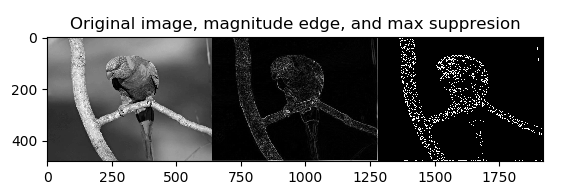
\includegraphics[width=0.8\textwidth]{pics/origMagNonMax}
    \caption{Comparison of original image, image with gradients and image with non max suppression}
    \label{fig:gradientsnonmax}
\end{figure}

\subsection{Corner detection}
The Harris Corner algorithm was implemented accourding to the steps from the lecture slides.

\subsubsection{myharris}
Simple implementation of the derivative operator like proposed: $[1, 0, -1]$

\pagebreak
\subsubsection{Evaluate myharris}
\begin{figure}[!htb]
    \centering
    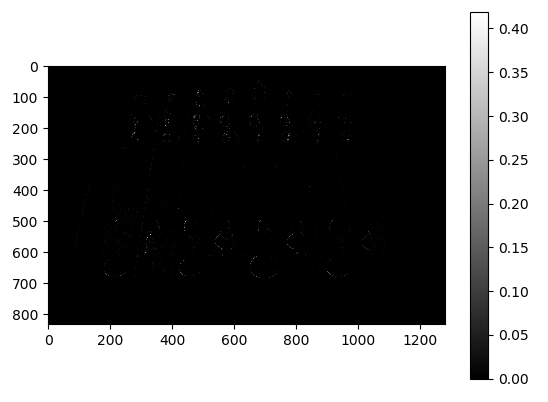
\includegraphics[width=0.5\textwidth]{pics/harris1}
    \caption{Output with low sigma of 0.2}
    \label{fig:harrissigma02}
\end{figure}

\subsubsection{Evaluate myharris rot 45$^{\circ}$}
\begin{figure}[!htb]
    \centering
    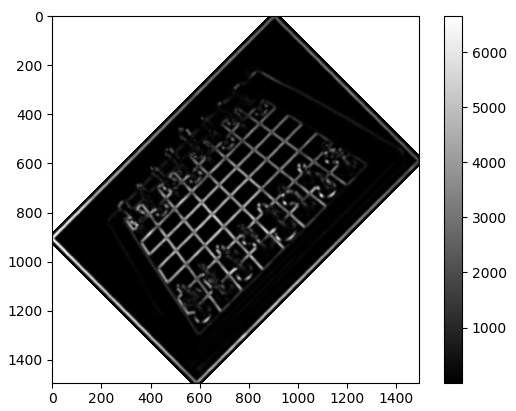
\includegraphics[width=0.5\textwidth]{pics/harris2}
    \caption{Output with simga of 6 and rotated 45$^{\circ}$}
    \label{fig:harrisrotated}
\end{figure}

\pagebreak

\subsubsection{Evaluate myharris downscaled}
\begin{figure}[!htb]
    \centering
    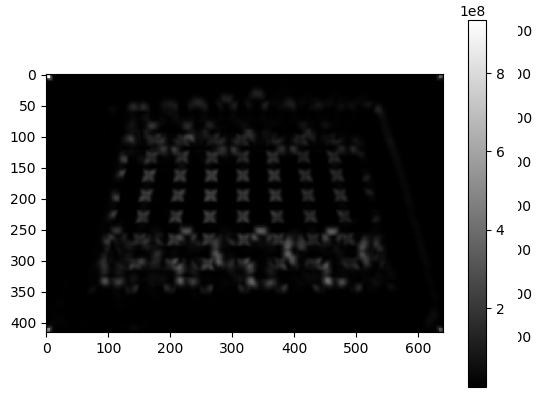
\includegraphics[width=0.5\textwidth]{pics/harris3}
    \caption{Output with simga of 6 and downscaled by 0.5}
    \label{fig:harrisdownscaled}
\end{figure}

\subsubsection{Harris Corner Properties}
The Harris Corner is a region, where a gradient goes in diferent directions. But these regions are difficult to
differentiate from edges with a high gradient in only one direction. It is invariant to scaling (as seen above)
because the structure matrix can be used for diagonal directions, better as from other gradients in x and y directions.

\section{Conclusion}
It was nice and a good training to implement all these 
algorithms by hand for once. Usually one would only use the 
from different frameworks provided algorithms without having
the actual knowledge how they really work.

\pagebreak


\end{document}